\documentclass[10pt,a4paper]{article}

\bibliographystyle{ieeetr}

\usepackage[margin=1in]{geometry}
\usepackage{graphicx}
\usepackage{subfig}
\usepackage{amsmath}
\usepackage{url}
\usepackage{pgfgantt}
\usepackage{lscape}
\usepackage{pdfpages}
% \usepackage{diagbox}

\graphicspath{{./figs/}}

\newcommand{\code}[1]{\texttt{#1}}

\title{A modular kernel for the Raspberry Pi: Progress Report}

\begin{document}

\maketitle

\begin{center}
    Thomas Archbold \\
    1602581 \\
    University of Warwick \\
\end{center}

\section{Introduction}
% problem that project addresses, motivations (importance of undertaking)
% make sure objectives are clear and clarify why it is a significant undertaking
% and of suitable level for third year project in computer science

\section{Background}
% all research I have put into it until this point - good understanding of
% background and how it fits into landscape (does not exist in isolation, before
% or after conception)
% indication of how background information was gained - a few citations that
% have been key sources for project

\section{Current progress}
The project is currently at a point at which the operating system is able to
successfully boot in the emulated environment provided by QEMU. Since it has
been capable of doing this since \code{boot.s} was written, early on in Term 1,
it is important to note the specific stages of initialisation performed by the
kernel at this point, as well as discuss the environment setup that has enabled
this point in development to be reached.

\subsection{Development environmet}
The project is being developed on a machine running Linux kernel version 4.16
onwards. Since the target environment, the Raspberry Pi 2 Model B, is different
to that on which it is being developed, a cross-compiler is required to compile
code that will run on the target machine, as opposed to the host. In particular,
available for download on the ARM developer website \cite{GNUtoolchain} is the
GNU Embedded Toolchain, which provides tools to target ARM Cortex family of
processors, including the GNU Compiler Collection (GCC). Conveniently this suite
of tools is available from Arch Linux's package manager, pacman \cite{pacman},
and this is the version of the cross-compiler used in the makefile.

Before writing any code, as the author had little-to-no prior experience in
systems programming, research had to be undertaken in order to get acquainted
with this environment. In particular, this involved skimming over the various
peripherals manuals, technical reference manuals, and programmer's guides for
programming on the Raspberry Pi to learn more about its hardware and how to
interface with it using ARM assembly. \cite{BCM2835} and \cite{BCM2836} detail the
peripherals on board the Raspberry Pi 2 Model B, the layout of their related
registers, and how to read and write them to do meaningful things with the
hardware, while \cite{TRM} and \cite{PG} provided help on ARM assembly's syntax,
and how and when to use specific instructions.

Particularly important so far have been the sections of the peripherals manual
on GPIO and UART, as until the implementation for the property mailbox interface
is working, all input and output is done through the serial connection provided
by the UART.  Since there were issues with getting the Pi to run on real
hardware, information about the GPIO peripheral was needed in order to write
basic low-level debugging functions, mainly in the form of getting the green ACT
LED to blink for various return values of functions.

\subsection{boot.s}
The first piece of code to be written was \code{boot.s}, which is responsible
for providing the basic setup of the entire system, which includes initialising
a minimum C environment. In particular, it sends three of the four cores on the
CPU to shutdown (to decrease overall complexity of the system, as discussed in
the specification), initialises the stack pointer at address \code{0x8000}, sets
up the BSS segment (where statically-allocated variables that are not explicitly
initialised are stored) and zeroes it out (as required by the C standard), and
then loads our C kernel entry point, \code{kernel\_main}, into memory to begin
its execution. Note that the Program Counter for the kernel starts at address
\code{0x8000} and grows upwards, so the stack can safely start at \code{0x8000}
without interfering with the kernel (as it grows downwards).

\subsection{linker.ld}
The code in \code{linker.ld} is responsible for linking all of the compiled
object files into one final executable. There are scripts which do this for
user-space programs, but since we are our own user-space, being the kernel, we
have to create one for ourselves. The various sections that the script defines
are as follows:
\begin{itemize}
    \itemsep0em
    \item \code{.text} - contains executable code
    \item \code{.rodata} - read-only data i.e. global constants
    \item \code{.data} - global variables initialised at compile-time
    \item \code{.bss} - uninitialised global variables
\end{itemize}

We also define the entry point of our entire operating system in this script,
namely the \code{\_start} routine from \code{boot.s}. This script also sets the
symbols \code{\_\_start} and \code{\_\_text\_start} to be \code{0x8000}, which
is where the bootloader will put the kernel image - the code from \code{boot.s}
will be put in the first part of this section, \code{.text.boot}. We use
\code{KEEP} to tell the compiler not to try to optimise the code in
\code{.text.boot}, and \code{ALIGN} sets the current address to the next
available page (the next address divisible by 4096). The \code{,rodata},
\code{.data}, and \code{.bss} sections are then declared in much the same way.

\subsection{Makefile}
The makefile was written to speed up the build process, and there are only a few
features to note. First is that here we specify that we are using the
\code{arm-none-eabi} toolchain, for the compiler to target the Raspberry Pi's
architecture as opposed to our own, in particular the Cortex-A7 processor. The
\code{-fpic} compilation flag is currently being used while we are ignoring the
Memory Management Unit, and in particular virtual memory, on the Pi, as it
creates position-independent code, and will keep separate applications from
interfering with each other within this single address space when processes are
implemented. The \code{-ffreestanding} compiler and linker flag, and the
\code{-nostdlib} linker flag, specifies that we are writing code in a
freestanding environment, and as such do not expect much of the C standard
library to exist, or for program startup to necessarily to be at \code{main()}.
Specifically, we only have access to the following header files:
\code{<float.h>}, \code{<iso646.h>}, \code{<limits.h>}, \code{<stdalign.h>},
\code{<stdarg.h>}, \code{<stdbool.h>}, \code{<stddef.h>}, \code{<stdint.h>}, and
\code{<stdnoreturn.h>}. The rest of the standard library must be implemented
ourselves.

\subsection{Atags}
The first piece of meaningful setup that can be done when the kernel is booted
is to get information about the memory available to the system. On the Raspberry
Pi, the bootloader creates creates a list of information about the hardware
called Atags, places it at address \code{0x100}, and passes it as the third
parameter to \code{kernel\_main} in register 2. Each tag in the list contains a
header consisting of two unsigned 32-bit values: the size of the tag (in 32-bit
words), and the tag value. Each header is then followed by information specific
to that tag, aside from \code{ATAG\_NONE}, which has no associated data, and
\code{ATAG\_CORE}, whose data is optional. To access the information in each of
the tags when we come across them, we must match the layout of each of the tags
\cite{atags} by defining appropriate C structs in \code{atag.h}.

To find the amount of memory on the device, we can skip through the Atags list
(using pointer arithmetic and information about the tag's size in its header)
until we come across the \code{ATAG\_MEM} tag. Then it is simply a case of
return the value in the \code{size} field of the \code{atag\_mem} struct.

\subsection{Initialising memory}
Throughout the operating system's execution, different processes will require
memory to perform computations. Although the only thing doing anything
meaningful at the moment is the kernel, which can theoretically use any memory
it wants, in order to impose some order for later implementations of processes
and user space, we split the available memory up into 4KiB pages. The total
number of pages is therefore given by the total amount of memory divided by the
page size.

\subsection{Printing to HDMI}
\subsection{Booting on real hardware}

% overview of work so far, including
%   technical content - what work have I done, meaningful summary of significant
%   aspects
%   progress - review progress against timetable. If unexpected delays, how have
%   they been dealt with?

\section{Next steps}
% outline plans for next term and any alterations to original ideas
% updated timetable with as much detail as possible

\section{Reflection}
% reflection and appraisal - assessment on how thing shave gone so far. Any
% lessons learned to make future progress smoother?

\section{Ethical consent}
% state that I have considered it, but not needed

\section{Project management}
% How have I managed the project so far - may use formal methodology (e.g.
% management of code versions), and can refer to less formal ways of keeping on
% track, e.g. regular meetings with supervisor

\bibliography{bibliography}

\appendix

% include project specification as part of appendices
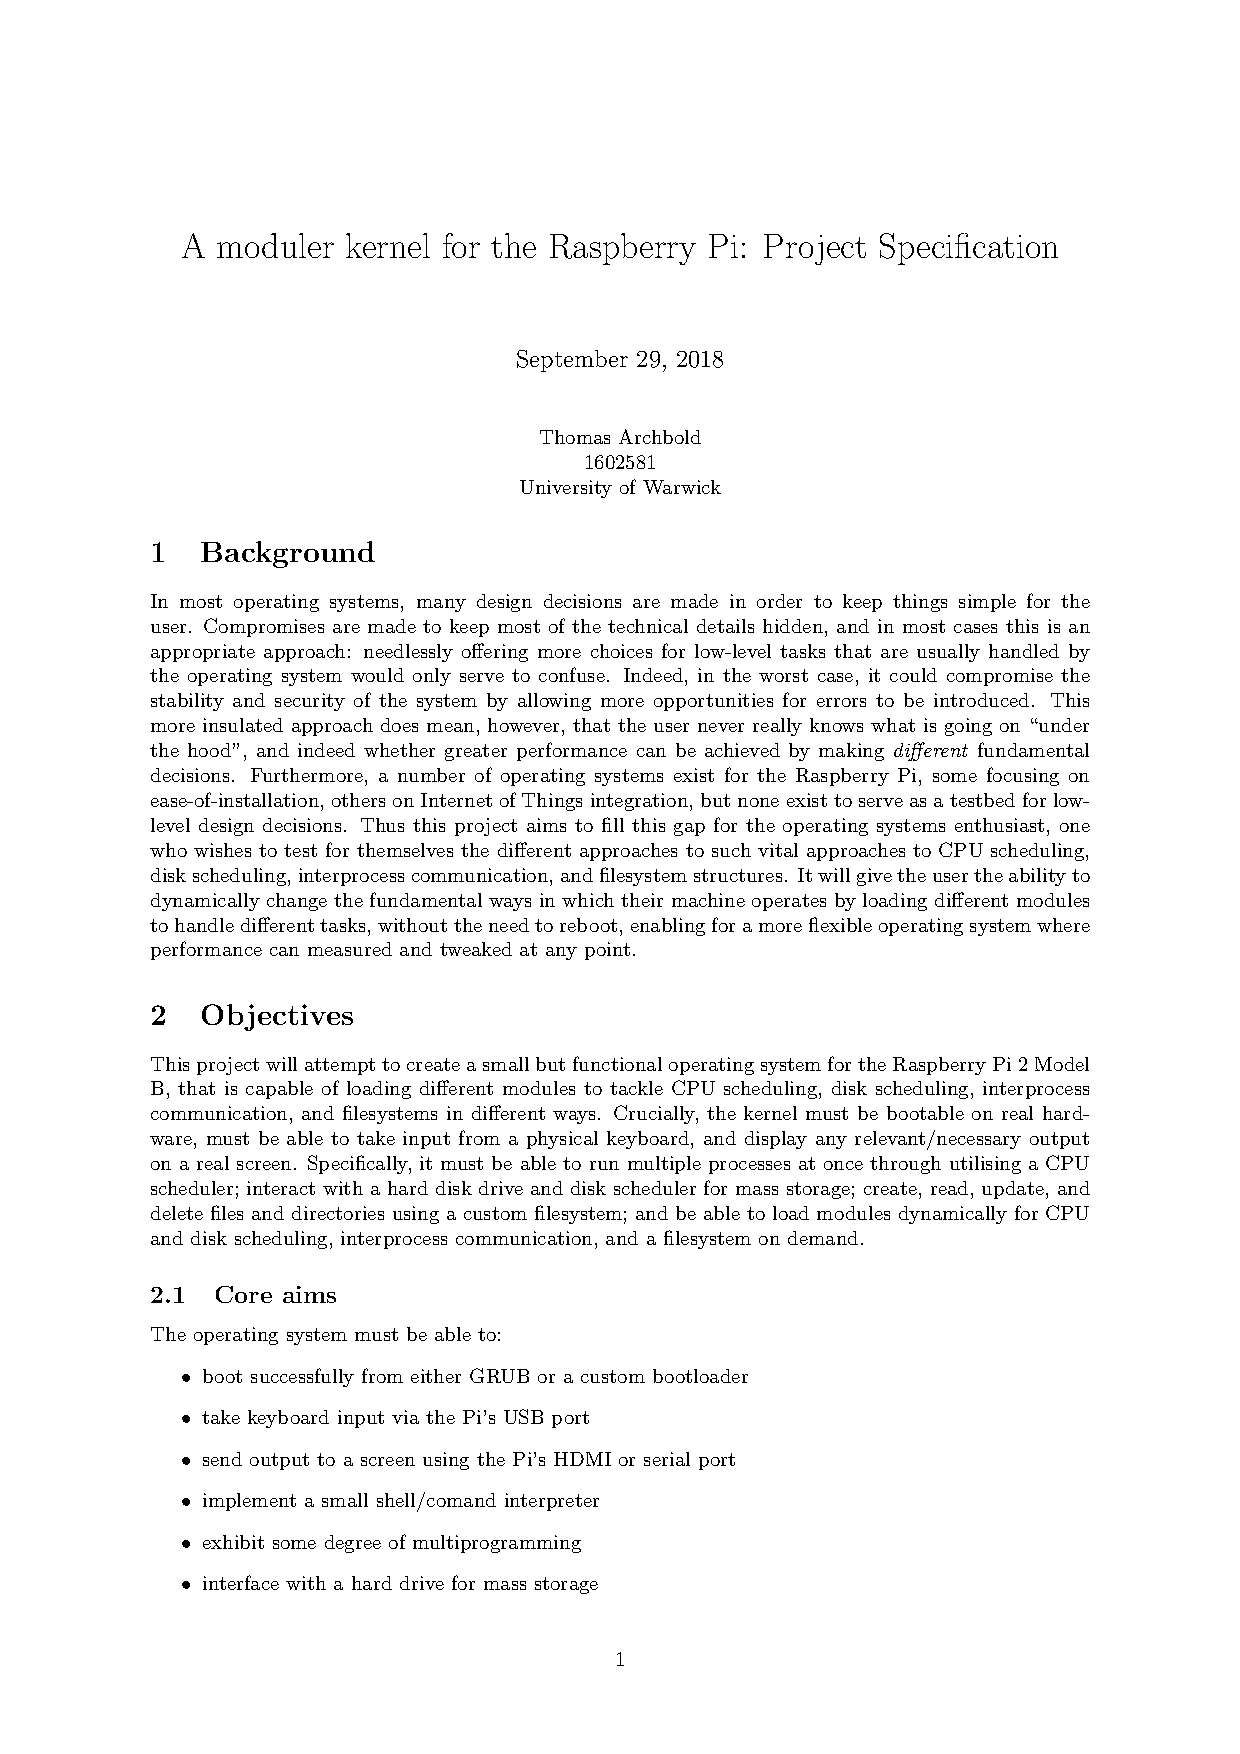
\includepdf[pages=-]{../specification/specification.pdf}

\end{document}
